\documentclass[10pt,conference,compsocconf]{latex-example-paper/IEEEtran}
\usepackage{booktabs}
\usepackage{amsmath}
\usepackage{url}
\usepackage{float}
\usepackage{graphicx}

\begin{document}
\title{Which Survey Answers Help Identify Reported Heart Disease?}
\author{Gustave Charles, Henri Jouneau, Vadim El Guedj}
\maketitle

\begin{abstract}
We predict whether a survey respondent reports a previous coronary heart disease diagnosis using the BRFSS dataset. Because only 8.8\% of respondents have a positive label, standard classification accuracy is misleading. Using pure NumPy implementations, we compare regularized logistic regression and ridge regression. We test the impact of feature selection, simple interaction terms, and decision threshold tuning. Adding questions on daily activity limitations and healthcare access improved validation F1 from 0.409 to 0.423. On our held-out test split, the selected logistic model achieves an F1 score of 0.428 and an AUC of 0.862.
\end{abstract}

\section{Introduction and data}
The supplied BRFSS dataset contains 328,135 labeled training respondents and 109,379 rows for test prediction. The binary label indicates a reported diagnosis of coronary heart disease, heart attack, or angina. Only 8.8\% of labeled rows are positive. A trivial classifier predicting ``no'' for every respondent achieves 91.2\% accuracy, but detects zero positive cases.

We therefore evaluate our models using positive-class F1 score (the harmonic mean of precision and recall) and the area under the ROC curve (AUC), which evaluates score ranking independent of a single cutoff. We use only the provided course data, with survey codes mapped according to the official BRFSS codebook \cite{cdc}.

\section{Methods and preprocessing}
\subsection{Model selection}
We compare two linear models implemented from scratch in NumPy: regularized logistic regression and ridge regression. Logistic regression is appropriate for binary classification because its sigmoid output produces values in $[0,1]$ and cross-entropy loss penalizes incorrect probabilities. Ridge regression serves as a linear baseline using mean squared error loss.

Both methods include an L2 penalty to stabilize weights across correlated survey answers. To ensure a direct comparison between the two objectives, both models are trained and tested on the exact same feature sets.

\subsection{Feature processing}
Our initial feature set included demographic variables (age, sex, BMI), general health ratings, several diagnosed conditions (stroke, kidney disease, diabetes), and basic lifestyle habits (smoking, exercise). We then added healthcare access indicators (insurance, personal doctor, medical costs), physical limitations in daily activities (difficulty walking, dressing, or running errands), and other diagnosed conditions (asthma, arthritis, depression). Finally, we added eight simple non-linear and interaction terms: squared terms for age and BMI, their product, and age multiplied by indicator variables for sex, high blood pressure, high cholesterol, diabetes, and smoking. These allow the linear model to capture age-dependent associations and non-linear trends.

For preprocessing, day-count questions with code 88 (zero days in the BRFSS codebook) were set to 0. Missing or invalid numerical entries were imputed with the training median, accompanied by an indicator column for missingness. Categorical questions were one-hot encoded; invalid or blank entries were encoded as all zeros. Numerical features were standardized to zero mean and unit variance using statistics computed solely on the training splits. The final design matrix contains 156 columns including the intercept.

\subsection{Validation strategy}
We set aside 20\% of the labeled data as an outer holdout set (seed 433, 65,627 rows). The remaining 80\% was split into training and development sets (80/20 split, seed 619). We used the development set to compare feature sets, regularization strengths, and iteration counts.

To prevent data leakage, all imputation medians, scaling parameters, and decision thresholds were fitted exclusively on training rows. The classification threshold was chosen to maximize F1 on training predictions rather than defaulting to 0.5.

\section{Results}
Table~\ref{tab:steps} shows the step-by-step ablation study on the development set. Adding questions about health context and physical limitations provided the largest single gain (F1 increased from 0.409 to 0.418). Adding polynomial and interaction terms provided only a slight additional gain (0.419). Increasing gradient descent training to 900 iterations (step size 0.5) improved convergence to 0.423. We evaluated L2 values of $10^{-5}$, $10^{-4}$, and $10^{-3}$, and selected $10^{-4}$.

\begin{table}[H]
\centering
\caption{Development F1 across feature and training choices.}
\label{tab:steps}
\begin{tabular}{lr}
\toprule
Logistic model configuration & F1 \\
\midrule
Original survey answers & .409 \\
Original + curved terms & .411 \\
Original + health and context & .418 \\
All answers + curved terms & .419 \\
All answers, 900 iterations & .423 \\
\bottomrule
\end{tabular}
\end{table}

On the outer holdout set (Table~\ref{tab:holdout}), the selected logistic model achieves an F1 of 0.428 and an AUC of 0.862, improving upon the initial logistic baseline (0.416 F1) and outperforming ridge regression on the same features (0.424 F1).

\begin{table}[H]
\centering
\caption{Held-out test results (F1 for the positive class).}
\label{tab:holdout}
\begin{tabular}{lrrr}
\toprule
Model & F1 & AUC & Accuracy \\
\midrule
Always ``no'' & .000 & .500 & .912 \\
Original logistic & .416 & .853 & .865 \\
Ridge (same 156 inputs) & .424 & .857 & .871 \\
Selected logistic & \textbf{.428} & \textbf{.862} & .867 \\
\bottomrule
\end{tabular}
\end{table}

The classification threshold has a significant impact on practical utility. With the standard 0.5 probability cutoff, the model detects only 14\% of respondents with heart disease. Selecting the cutoff that maximizes training F1 increases recall to 56\%, at the cost of more false positives (Figure~\ref{fig:pr}).

\begin{figure}[H]
\centering
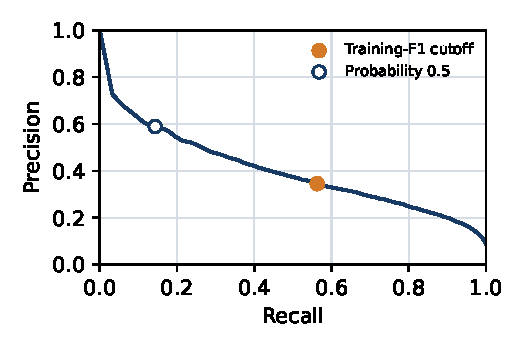
\includegraphics[width=\columnwidth]{figures/precision_recall.pdf}
\caption{Precision-recall curve on the holdout set. Points mark the default 0.5 probability cutoff and the F1-optimized cutoff.}
\label{fig:pr}
\end{figure}

\newpage
\section{Discussion and limitations}
The experimental comparisons show that questions reflecting mobility limitations and general health provide the largest predictive gains, whereas non-linear terms provide only modest improvements. Many survey answers carry overlapping signal, with age, general health, and mobility capturing most of the predictive pattern.

Several limitations should be noted. At the F1-optimized threshold, roughly two out of three positive alerts are false alarms, even though the model detects more than half of the true positive cases. Furthermore, sensitivity varies substantially across age groups: the model identifies 64\% of positive respondents aged 65 and older, but only 20\% of positive respondents under 50. In addition, the target variable reflects a past, self-reported diagnosis rather than prospective risk of a future event; the model should therefore not be interpreted as a clinical diagnostic tool. Finally, our local model selection relied on a single train/development split and one holdout set rather than repeated cross-validation.

On AIcrowd, our final submission obtained an F1 score of 0.438 and an AUC of 0.880. All validation tables can be reproduced with \texttt{python3 run.py --validate}, and final test predictions are generated via \texttt{python3 run.py}.

\begin{thebibliography}{1}
\bibitem{cdc} Centers for Disease Control and Prevention, ``2015 BRFSS Codebook,'' \url{https://www.cdc.gov/brfss/annual_data/2015/pdf/codebook15_llcp.pdf}.
\end{thebibliography}
\end{document}
